% chap5.tex
\chapter[
洗浄条件の違いがウイルス除去効率に及ぼす影響
]{
洗浄条件の違いがウイルス除去効率\\\hspace{4.1em}に及ぼす影響実験の基礎的検討
}
%--------------------------------------------------

\section{本章の目的}
第4章では、清浄な水500\,mLを用いた単回洗浄により、
掌表面に付着したMS2ファージのうち約12～33\%が残存することが明らかとなった。
この結果は、500\,mLという限られた水量であっても一定の洗浄効果が得られる一方、
完全な除去には至らないことを示している。

一方、災害時や水資源が制限される状況では、
洗浄に使用できる水量そのものをできる限り抑えることが求められる。
そのため、総水量を一定とした場合に、
洗浄方法（単回洗浄か分割洗浄か）の違いが
ウイルス除去効率にどのような影響を及ぼすのかを検討することは、
実用上重要な課題である。

そこで本章では、
洗浄水量を1回あたり100\,mLとし、
洗浄回数を1～5回に分割した条件下で掌洗浄を行い、
各洗浄回数後のMS2ファージ残存率を算定・比較することで、
分割洗浄の有効性および節水効果について基礎的に検討することを目的とした。

%--------------------------------------------------

\section{実験方法}

\subsection{分割洗浄条件}
本実験は被験者5名を対象として実施した。
各被験者について右手および左手を対象とし、
第4章と同一条件でMS2ファージ懸濁液への浸漬操作を行った後、
洗浄条件のみを変更した。

洗浄は、
1回あたり100\,mLの清浄水を用い、
最大5回まで繰り返し実施した。
すなわち、
総洗浄水量は最大500\,mLとし、
洗浄回数を1～5回に分割した条件で、
各回の洗浄後に洗浄水を回収した。

%--------------------------------------------------
\newpage
\section{残存率の算定方法（分割洗浄条件）}
初期付着ファージ量の算定方法は、
第4章で示した方法と同一とした。
すなわち、
MS2ファージ懸濁液の初期濃度 $C_0$（PFU/mL）、
単位面積あたりの水分付着量 $W$（mL/cm$^2$）、
および各被験者の掌面積 $A$（cm$^2$）から、
初期付着ファージ量 $N_0$（PFU）を算定した。

分割洗浄条件においては、
各洗浄回後に回収された洗浄水中のファージ濃度を測定し、
以下の手順で累積回収量を算定した。

\begin{itemize}
  \setlength{\itemsep}{0pt}
  \setlength{\parskip}{0pt}
  \setlength{\topsep}{0pt}
  \item 1回目洗浄後：
  洗浄水中のファージ濃度に100\,mLを乗じ、
  回収量を算定し、これを累積回収量とした。
  \item 2回目以降：
  各回の洗浄水中ファージ濃度に100\,mLを乗じて得られた回収量を、
  それまでの累積回収量に加算した。
  \item 5回目まで同様の操作を行い、
  各洗浄回後の累積回収量を算定した。
\end{itemize}

各洗浄回数後の残存率 $R_x$（\%）は、
$x$回目までの累積回収量 $N_{\mathrm{rec},x}$ を用いて、
次式により算定した。

\begin{equation}
R_x = \left(1 - \frac{N_{\mathrm{rec},x}}{N_0}\right) \times 100
\end{equation}

この残存率は、
分割洗浄条件下において
掌表面に残存するMS2ファージ量の割合を示す指標として用いた。

%--------------------------------------------------

\section{結果および考察}

\subsection{分割洗浄条件下における残存率の変化}

\begin{figure}[H]
  \centering

  \begin{minipage}{0.48\linewidth}
    \centering
    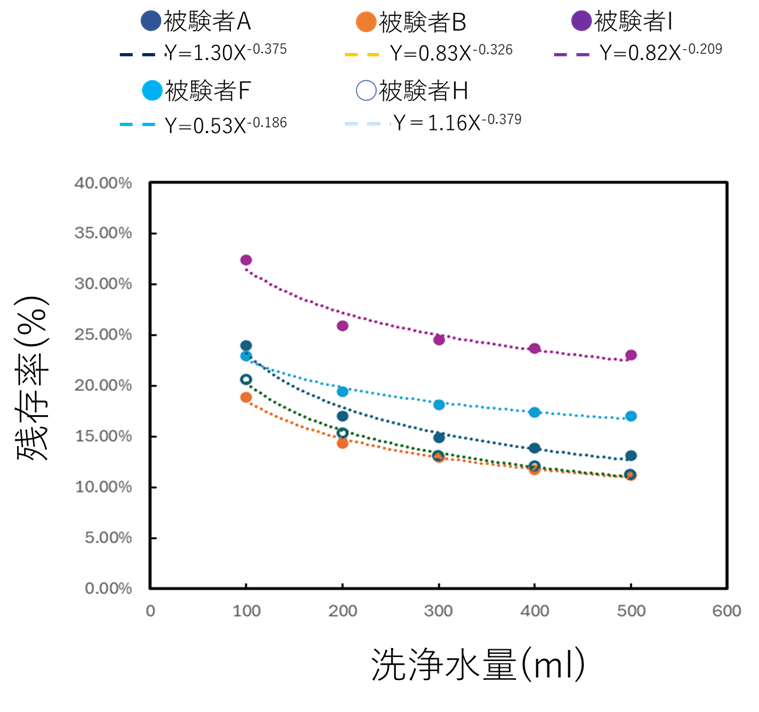
\includegraphics[width=\linewidth]{fig/right_hand_residual.png}
    \caption*{(a) 右手}
  \end{minipage}
  \hfill
  \begin{minipage}{0.48\linewidth}
    \centering
    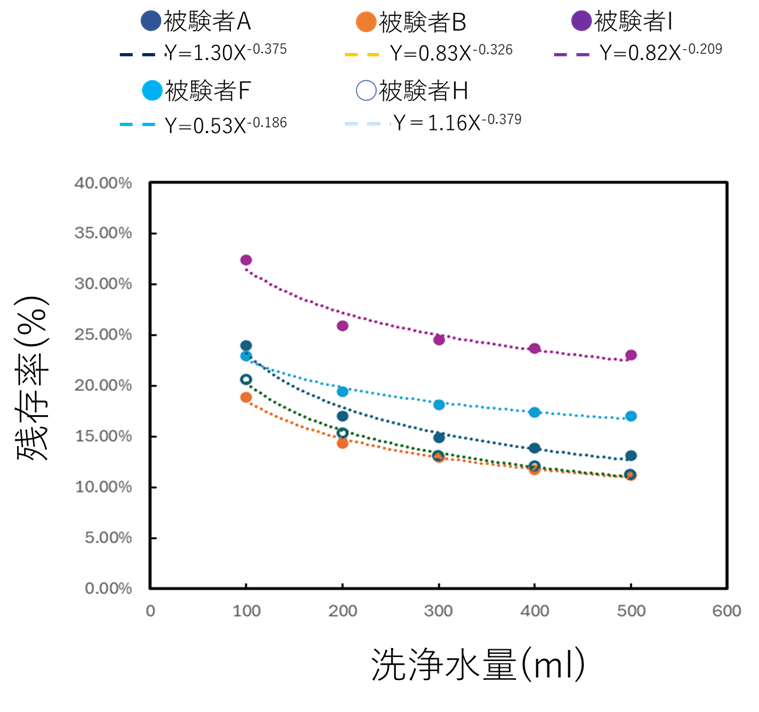
\includegraphics[width=\linewidth]{fig/left_hand_residual.png}
    \caption*{(b) 左手}
  \end{minipage}

  \caption{%
    分割洗浄条件下における洗浄水量（累積）とMS2ファージ残存率の関係\\
    （被験者5名における右手および左手の結果）
  }
  \label{fig:split_wash_residual}
\end{figure}

図\ref{fig:split_wash_residual}に、
被験者5名における分割洗浄条件下での
洗浄水量（累積）とMS2ファージ残存率の関係を、
右手および左手それぞれについて示す。

いずれの被験者および手においても、
洗浄水量の増加に伴い残存率は低下する傾向を示した。
特に、初回（100\,mL）から200～300\,mL程度までの洗浄においては、
残存率の低下が比較的大きく、
それ以降は低下幅が緩やかになる傾向が認められた。

この結果は、
初期洗浄によって掌表面から除去されやすいファージが
優先的に除去され、
その後は皮膚表面のしわや溝などに残存したファージが
除去されにくくなる可能性を示唆している。

また、
同一の洗浄条件下であっても被験者間で残存率の絶対値には差がみられ、
第4章で示した個人差が
分割洗浄条件下においても一定程度存在することが確認された。
一方で、
右手と左手を比較すると、
被験者によっては一方の手で残存率がやや高い傾向を示す場合があったが、
全体としては左右で共通した低下傾向が認められた。

これらの結果から、
分割洗浄による残存率の低下挙動は、
個人差や左右差よりも、
洗浄水量（累積）に強く依存していることが示唆された。


\subsection{分割洗浄の有効性と節水効果}
以上の結果より、
総洗浄水量が同一であっても、
洗浄回数を分割することで、
段階的にファージを除去できることが示された。
特に、
100～300\,mL程度の比較的少ない水量でも、
一定の除去効果が得られることは、
節水を考慮した洗浄方法として有用であると考えられる。

一方で、
洗浄回数を増やしても残存率の低下が頭打ちとなる傾向も確認されており、
水量や洗浄回数には効率的な範囲が存在する可能性が示唆された。
本章の結果は、
次章におけるリスク評価において、
現実的な洗浄条件を設定するための基礎情報として活用される。

%--------------------------------------------------

\section{本章のまとめ}
本章では、
被験者5名を対象に、
洗浄水量を100\,mLずつ分割した洗浄条件下で
MS2ファージの残存率を評価した。
その結果、
洗浄水量の増加に伴い残存率は低下するものの、
低下幅は洗浄初期で大きく、
その後は緩やかになる傾向が認められた。

分割洗浄は、
少ない水量でも一定の除去効果を得られる可能性を示しており、
節水を考慮した手指洗浄方法として有効であると考えられる。
本結果は、
後続章における感染リスク評価の前提条件として重要な知見を提供する。
